\chapter{Desenvolvimento do trabalho}

% Apresentar os resultados das fases que transformam
% os requisitos em produtos finais.
% • A estrutura desse capítulo depende do processo de
% desenvolvimento do trabalho.
% • A organização e as seções desse capítulo devem ser
% definidas juntamente com o orientador.

Este capítulo tem como objetivo explicitar quais foram as decisões de projeto que foram tomadas ao longo do desenvolvimento do sistema.

\section{Tecnologias utilizadas}
O projeto pretende definir algumas tecnologias de base para serem usadas durante o desenvolvimento de cada fase dele.

    \subsection{Conexão OBD-II}
A integração do OBD-II (On-Board Diagnostics) neste projeto de rastreamento de veículos representa um avanço significativo na obtenção de dados precisos e abrangentes sobre o desempenho do veículo. O OBD-II, um padrão presente em muitos veículos modernos, fornece acesso a uma variedade de parâmetros, como velocidade, rotações por minuto (RPM), temperatura do motor, e códigos de diagnóstico de falhas. Ao conectar o sistema de rastreamento ao conector OBD-II do veículo, é possível extrair informações em tempo real sobre a condução, condições do motor e possíveis problemas mecânicos.

Já existe uma plataforma aceleradora desenvolvida no GitHub que consegue
comunicar-se com o veículo através do protocolo OBD-II\textsuperscript{[12]}. Esse outro projeto
implementa o protocolo OBD-II e também uma interface gráfica básica para mostrar
os dados fornecidos pelo carro.

A figura \ref{fig:obd2_plataforma} mostra uma plataforma onde é possível ver alguns dos dados quando o motorista estava dando uma volta ao redor do bairro.

    \begin{figure}[hp]
    \centering
    
    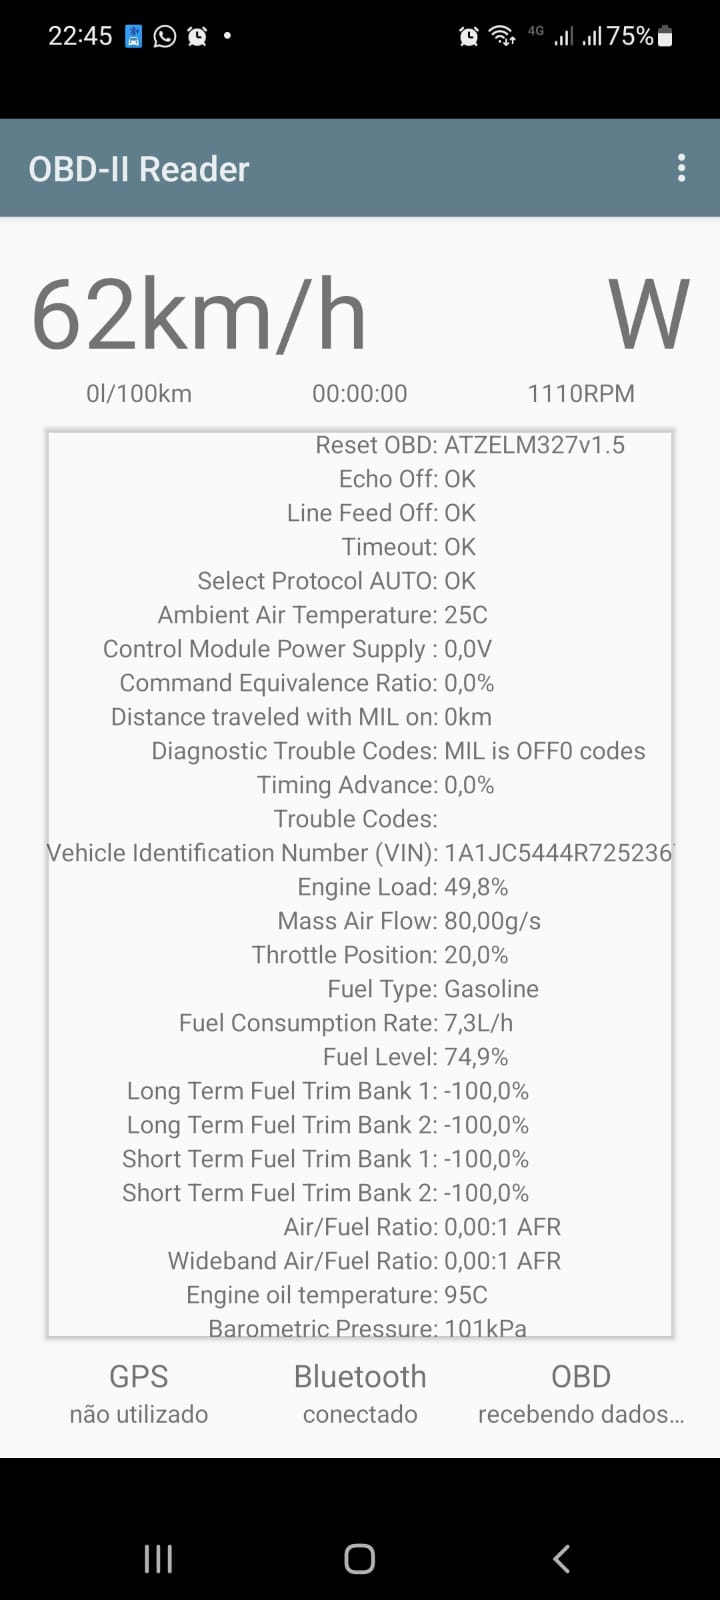
\includegraphics[scale=0.3]{figures/obd2.jpg}
    
    \caption{Interface básica com porta OBD-II\textsuperscript{[12]}}.
    
    \label{fig:obd2_plataforma}
\end{figure}
    
    \subsection{Android Studio} A utilização da IDE Android Studio neste projeto de rastreamento de veículos desempenha um papel central no desenvolvimento de aplicativos móveis dedicados à interação com o sistema. O Android Studio, sendo a principal ferramenta de desenvolvimento para aplicativos Android, oferece um ambiente integrado e robusto que simplifica a criação, teste e depuração de software. 
    
    A plataforma fornece recursos avançados de design de interface do usuário, facilitando a criação de aplicativos intuitivos e visualmente atraentes para os usuários finais. A integração perfeita com o Android SDK (Software Development Kit) permite o acesso às APIs e recursos específicos do sistema operacional Android, garantindo uma implementação eficiente de funcionalidades como a transmissão Bluetooth, a visualização de dados de rastreamento e a interação em tempo real. Além disso, as ferramentas de emulação e depuração incorporadas no Android Studio simplificam o processo de teste em diferentes dispositivos, contribuindo para a criação de aplicativos estáveis e adaptáveis.

     \begin{figure}[hp]
    \centering
    
    
\includegraphics[scale=0.4]{figures/logo_android.png}
    
    \caption{Logo Android Studio}.
    
\end{figure}
    
     \subsection{Banco de dados} A integração do MySQL e do AWS RDS (Relational Database Service) em um projeto de rastreamento de veículos é uma estratégia robusta para o gerenciamento eficiente e escalável dos dados do sistema. O MySQL, um sistema de gerenciamento de banco de dados relacional de código aberto, proporciona uma estrutura confiável para armazenar e organizar informações como histórico de rotas e dados do OBD-II. 
     
     Ao escolher o AWS RDS como a plataforma de hospedagem para o MySQL, ganha-se os benefícios adicionais de escalabilidade automática, alta disponibilidade e segurança avançada oferecidos pela infraestrutura em nuvem da Amazon. A integração dessas tecnologias permite o acesso eficiente aos dados, consultas rápidas e uma gestão simplificada do banco de dados. Além disso, o AWS RDS lida com tarefas operacionais, como backup automático e manutenção, permitindo que os desenvolvedores concentrem seus esforços em aprimorar as funcionalidades do sistema de rastreamento. 
     
     Essa combinação proporciona uma base sólida para o armazenamento e recuperação de dados, promovendo a confiabilidade e eficácia do sistema de rastreamento de veículos.

      \begin{figure}[hp]
    \centering
    
    
\includegraphics[scale=0.4]{figures/logo_Mysql.jpg}
    
    \caption{Logo do Mysql}.
    
\end{figure}

    
     \subsection{\textit{Python} e Folium} A junção do Python e do Folium em um projeto de sistema de coleta de dados oferece uma poderosa combinação para a visualização interativa e geoespacial dos dados. O Folium é uma biblioteca Python que simplifica a criação de mapas interativos baseados na web, utilizando a infraestrutura do Leaflet.js. Integrar o Folium ao projeto permite que os desenvolvedores gerem mapas dinâmicos que destacam informações específicas relacionadas ao rastreamento de veículos.

    Essa integração Python-Folium é particularmente útil para análises geoespaciais em sistemas de rastreamento de veículos, proporcionando uma representação geográfica e visualmente intuitiva dos dados de telemetria. Além disso, a flexibilidade do Python permite a personalização dos mapas e a incorporação de recursos adicionais conforme as necessidades específicas do projeto, contribuindo para uma interface de usuário mais informativa e envolvente.

      \begin{figure}[hp]
    \centering
    
    
\includegraphics[scale=0.1]{figures/python_folium.jpg}
    
    \caption{Logo Python + Folium }.  
\end{figure}

% interface com usuario, banco de dados, conexão obd2


\section{Projeto e implementação}
Esta seção descreverá as decisões feitas durante o trabalho.

Para criar os mapas do aplicativo, foi utilizado o framework Folium. A biblioteca Folium é uma poderosa ferramenta para manipular e visualizar dados geoespaciais usando Python. Com o Folium, é possível criar mapas interativos personalizados e incorporar dados neles de várias maneiras. Para manipular dados usando o Folium, pode-se começar importando a biblioteca e criando um objeto Map que representa o mapa. 

Em seguida, pode-se adicionar camadas, como marcadores, polígonos e popups, para exibir dados de forma intuitiva no mapa. Além disso, o Folium permite a integração de dados geoespaciais em diferentes formatos, como GeoJSON, tornando-o uma ferramenta flexível para análise e visualização de dados geoespaciais em Python.

A figura \ref{fig:python_libs} mostra as bibliotecas utilizadas para desenvolver o mapa:

\begin{figure}[hp]
    \centering
    
    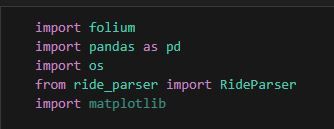
\includegraphics[scale=0.8]{figures/bibliotecas.jpg}
    
    \caption{Bibliotecas utilizadas para gerar o mapa da rota.}
    
    \label{fig:python_libs}
\end{figure}

        % \begin{center}
        %  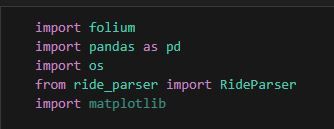
\includegraphics[scale=0.8]{figures/bibliotecas.jpg}
        %  
        %  \end{center}

A função da classe RideParser é analisar dados dos trajetos.A classe pode receber dados de entrada que descrevem o destino, e então analisa esses dados para extrair informações úteis. Como, por exemplo, traçar a rota feita pelo automóvel. Já o módulo 
''os'' fornece funcionalidades relacionadas ao sistema operacional, permitindo que você interaja com o ambiente do sistema, como manipular diretórios, arquivos, obter informações sobre o sistema, manipular variáveis de ambiente, entre outras tarefas relacionadas ao sistema operacional.
Por fim, tanto a biblioteca pandas, como a matplotlib foram utilizadas para manipular os dados.

Para traçar uma trajetória no mapa usando a biblioteca Folium em Python, será necessário uma lista de pontos de latitude e longitude que representam a trajetória. A partir dos pontos de latitude e longitude colhidos dos sensores do celular, cria-se uma lista de coordenadas que representam os pontos da trajetória. Em seguida, criamos um objeto de mapa usando o Folium e é adicionado uma linha de trajetória (um polilinha) que conecta os pontos da lista e o mapa pode ser visualizado. Uma demonstração de uma trajetória pode ser vista na figura \ref{fig:car_route_1}.

\begin{figure}[hp]
    \centering
    
    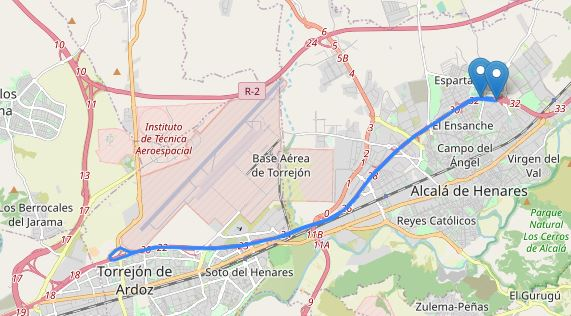
\includegraphics[scale=0.8]{figures/rota_1.jpg}
    
    \caption{Rota de uma das viagens fornecidas pelo \textit{UAH Driveset}.}
    
    \label{fig:car_route_1}
\end{figure}

A visualização de um vídeo que apresenta o trajeto do veículo sincronizado com um gráfico de aceleração proporciona uma compreensão visual e analítica aprimorada do comportamento de condução. Este recurso permite aos usuários acompanhar de forma imersiva o percurso do veículo enquanto simultaneamente observam as variações na aceleração ao longo do tempo. 

Ao visualizar o vídeo, os usuários podem identificar eventos específicos, como curvas acentuadas, frenagens bruscas ou acelerações rápidas, correlacionando-os diretamente com os picos e quedas no gráfico de aceleração exibido ao lado. Essa abordagem oferece uma representação mais holística da experiência de condução, permitindo uma análise detalhada de como o estilo de direção afeta diretamente a aceleração do veículo. 

Além disso, essa visualização combinada pode ser uma ferramenta valiosa para treinamento de motoristas, análise de incidentes e feedbacks personalizados, proporcionando uma compreensão mais rica e envolvente do desempenho do veículo e do comportamento do condutor.
A figura \ref{fig:rota1integrante} mostra o video e o grafico da aceleração.

\begin{figure}[hp]
    \centering
    
    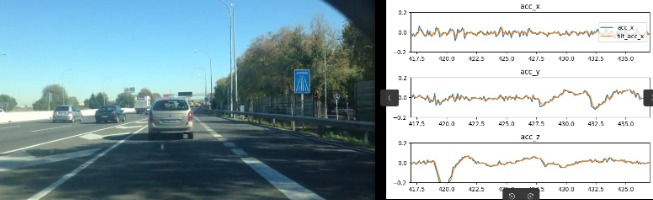
\includegraphics[scale=0.3]{figures/rota_integrante.jpg}
    
    \caption{Rota de uma viagem de um dos integrantes do grupo}.
    \label{fig:rota1integrante}
\end{figure}

\section{Testes e avaliação}
% descrever o plano de testes do sistema: testes de software, modulo, integração e validação
Alguns testes abstratos e macroscópicos podem ser definidos já antes de o projeto começar:

\begin{itemize}
    \item \textbf{Conferir conexão OBD-II:} conectar o dispositivo de leitura na entrada do carro e fazer um \textit{Hello World} através do aplicativo de conexão, mostrando que o protocolo está sendo feito da forma correta.
    
    \item \textbf{Teste de continuidade de transferência de dados:} andar com o carro por alguns minutos e atestar que nenhum dado foi perdido por falta de conexão.
    
    \item \textbf{Equivalência de envio e recepção de dados:} comparar o \textit{log} de envio de dados do aplicativo de interface com a porta OBD-II com o \textit{log} de salvamento do banco de dados hospedado na nuvem; a quantidade de dados, os \textit{timestamps} deles e seus conteúdos devem ser idênticos. 
    
    \item \textbf{Testes de segurança:} de forma bastante ampla, ratificar que não é possível ter acesso aos dados de um certo usuário sem ter as informações de \textit{login}.
    
    \item \textbf{Geração de dados \textit{outliers}:} para verificar se o sistema descarta corretamente as informações que fogem totalmente do padrão esperado ou se consegue pelo menos esconder isso do usuário, para que o \textit{dashboard} mantenha-se com dados consistentes e "limpos", isto é, sem que mostrem números surpreendentes, mas falsos, para o usuário final.
    
\end{itemize}

\section{Dependências do Gradlle}

Em um primeiro instante o app android-obd-reader não queria rodar na IDE Android studio. Para que isso fosse possível foi necessario fazer alterações no arquivo \textbf{gradle/wrapper/gradle-wrapper.properties}. Atualizar as dependências do Gradle  é muitas vezes necessário para garantir que o seu aplicativo possa se beneficiar das correções de bugs, melhorias de desempenho e novos recursos fornecidos pelas versões mais recentes das bibliotecas que você está utilizando. Este link \url{https://github.com/APF2000/android-obd-reader-pires/commit/def70ed262b1fad28cc9e2b98a48af45cfac5695} mostra as alterações que foram necessárias.


% Using \texttt{biblatex} you can display a bibliography divided into sections, depending on citation type. 
% Let's cite! Einstein's journal paper \cite{einstein} and Dirac's book \cite{dirac} are physics-related items. 
% Next, \textit{The \LaTeX\ Companion} book \cite{latexcompanion}, Donald Knuth's website \cite{knuthwebsite}, \textit{The Comprehensive Tex Archive Network} (CTAN) \cite{ctan} are \LaTeX-related items; but the others, Donald Knuth's items, \cite{knuth-fa,knuth-acp} are dedicated to programming. 

